\section{Grundlagen}
Diese Vorlage soll den Studenten im Studiengang Elektro- und Informationstechnik den Einstieg in \LaTeX\ vereinfachen und anhand von Beispielen \textbf{(siehe direkt im tex-File)} einige Tipps und Tricks auf den Weg geben. Zudem wird auch auf Vorgaben eingegangen, welche für eine technische Dokumentation wichtig sind und sicherstellen, dass alle Dokumentationen des Studiengangs gleich designed werden. Für \LaTeX "~Neulinge wird das Dokument \emph{LaTeX2e-Kurzbeschreibung} (siehe \cite{l2kurz}) empfohlen.  Die elektronische Datei ist im Ordner \mbox{\emph{/bibliography/}} zu finden. Daraus stammt auch das folgende Zitat:
\begin{quote}
Typographisches Design ist ein Handwerk, das erlernt werden muss. Ungeübte Autoren machen dabei oft gravierende Fehler. Fälschlicherweise glauben viele Laien, dass Textdesign vor allem eine Frage der Ästhetik ist -- wenn das Schriftstück vom künstlerischen Standpunkt aus \enquote{schön} aussieht, dann ist es schon gut \enquote{designed}. Da Schriftstücke jedoch gelesen und nicht in einem Museum aufgehängt werden, sind die leichtere Lesbarkeit und bessere Verständlichkeit wichtiger als das schöne Aussehen. \cite{l2kurz}
\end{quote}

\subsection{Teamfähige Installation}

Bei der Arbeit mit \LaTeX{} empfiehlt es sich sehr, dass alle im Team dieselbe Version installiert haben.  Am einfachsten ist das mit einer Installation von \url{https://tug.org/texlive/}.  Dies ist eine nahezu vollständige Installation von allem was es braucht, so aufbereitet, dass die Dateiversionen zusammenpassen, und lauffähig auf Linux, MacOS und Windows.

\subsection{Grundgerüst}
Um ein \LaTeX-Dokument zu erstellen braucht es eigentlich nicht viel, nur eine Textdatei mit der Dateiendung \texttt{.tex}, welche mit dem Befehl \verb|\documentclass[]{}| beginnt und die Umgebung \verb|\begin{document}| \dots \verb|\end{document}| enthält.
Darin kann nun die ganze Dokumentation erstellt und kompiliert werden, jedoch wird das schnell unübersichtlich und eignet sich sehr schlecht für das gemeinsame Arbeiten am Dokument.

Durch das "`Outsourcen"' von zusammengehörenden Blöcken (z.\,B. ganze Kapitel) in externe Dateien kann eine \textbf{übersichtliche und teamfähige Struktur} geschaffen werden. Damit sie bei der Kompilation des Dokuments beachtet werden, müssen sie in der Masterdatei eingebunden werden.
Einerseits wird der Befehl \verb|\input{}| dazu verwendet, Texte \textbf{1:1} aus einer Datei einzubinden. Dies kann beispielsweise dazu dienen, die Dokumenteinstellungen und Packages aus einer externen Datei (hier \mbox{\texttt{header.tex}}) zu laden.\footnote{Beim Kompiliervorgang wird das aktuelle \texttt{.aux}"~File weitergeführt.}
Andererseits können ganze Kapitel mit \verb|\include{}| eingebunden werden. Dieser Befehl fügt ein zusätzliches \verb|\clearpage| \textbf{vor} und \textbf{nach} dem geladenen Text hinzu. Dadurch wird sichergestellt, dass ein Seitenumbruch am Anfang und Schluss gesetzt und die Gleitobjekt"=Warteschlange geleert wird.\footnote{Für das eingefügte Kapitel wird ein separates \texttt{.aux}"~File erzeugt.} Zu beachten ist, dass der \verb|\include{}|"~Befehl nur in der Masterdatei benutzt wird, da er nicht verschachtelt werden kann. 

In Abbildung~\ref{fig:Struktur} ist die Struktur des aktuellen \LaTeX-Projekts aufgezeigt.\\
\textbf{Diese Struktur ist als Minimalstruktur zu verstehen und ist für Berichte des Studiengangs EIT vorgeschrieben!}

\clearpage 

Die Ordner sind für folgende Dateien vorgesehen:
\begin{tabbing}
\quad \= \verb|appendix/| \qquad \= im Anhang eingebundene Dokumente oder Bilder\\
      \> \verb|graphics/|        \> Grafiken (vorzugsweise als Vektorgrafik -- pdf)\\
      \> \verb|literature/|      \> zitierte Dokumente, Paper, Webseiten und die Bibliographie-Datenbank\\
      \> \verb|sections/|        \> mit \verb|\include{section.tex}| eingefügte Kapitel\\
      \> \verb|tikz/|            \> tikz-Grafiken (Standalone-Modus) zum Einbinden mit \verb|\section{Tikz-Grafiken}
Tikz ist ebenfalls sehr mächtig und auf den ersten Blick auch sehr kompliziert. Schon alleine die Dokumentation des Grundpackages erstreckt sich über 1000 Seiten. Tikz lohnt sich vor allem, wenn die erstellte Grafik (oder nur Teile davon) wiederverwendet werden können.
Es folgen drei Beispiele für Tikz-Grafiken.

Man beachte, dass diese in einem eigenen \enquote{\LaTeX-Projekt} erstellt wurden. Dieses hat die \verb|\documentclass{standalone}| und kann deswegen eigenständig kompiliert werden. Dabei werden automatisch Unterstüzungslinien/Grid eingeblendet (wurde programmiert), welche die Gestaltung der Grafik extrem erleichtern. Schaut euch doch die Tikz-Dateien an und kompiliert sie separat, es lohnt sich!

Mittels Befehl \verb|\includestandalone{}| werden dann diese in jedes andere Projekte eingebunden, und zwar nicht als PDF sondern direkt erstellt beim Kompilieren.

Somit können wir nun einfache elektrische Schaltungen wie in Figur~\ref{subfig:einfach} oder auch komplizierte Blockschaltbilder wie in Figur~\ref{subfig:kompliziert} programmieren.

\begin{figure}[b]
\centering
\subfloat[Einfach]{\includestandalone{tikz/beispiel1}\label{subfig:einfach}}

\subfloat[Kompliziertes Blockschaltbild]{\includestandalone{tikz/beispiel2}\label{subfig:kompliziert}}

\caption{Zwei tikz-Beispiele: \protect\subref{subfig:einfach} einfach, \protect\subref{subfig:kompliziert} kompliziert.}
\label{fig:tikz}
\end{figure}

Im Dokumenteordner \mbox{\emph{/tikz/}} findet ihr noch zwei weitere Beispiele. Eines zeigt ein \textbf{animiertes Tikz} und das andere interagiert mit \textbf{gnuplot}, um Plots zur Laufzeit zu erstellen. Um gnuplot nutzen zu können sind ein paar zusätzliche Installationen notwendig. Weiter muss der Kompilierbefehl für \texttt{pdflatex} mit \texttt{--shell-escape} erweitert werden. Das Internet bietet gute Unterstützung bei der Integration von gnuplot.
Viele weitere coole Beispiele findet ihr auf \mbox{http://www.texample.net/tikz/examples/}.

|\\
      \> \verb|versions/|        \> Ablage für verschiedene Dokumentversionen (z.\,B. bei Abgabe)
\end{tabbing} 

\begin{figure}
\centering
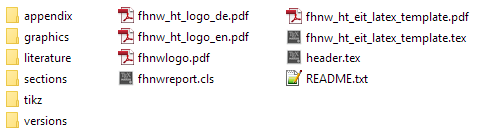
\includegraphics[width=0.8\linewidth]{ordner_struktur.png}
\caption{Minimalstruktur des \LaTeX -Projekts.}\label{fig:Struktur}
\end{figure}

\subsection{Packages}
Packages können dem Benutzer helfen, gewisse Dinge einfacher zu Programmieren, indem vorgefertigte Funktionen geladen werden. Dies ist zwar nützlich, sollte jedoch mit Vorsicht genossen werden.
\textbf{Unterschiedliche Packages können einander gegenseitig beeinflussen und dadurch unerklärliche Fehler verursachen. Aus diesem Grund empfiehlt sich, nur wirklich verwendete Packages dem Header hinzufügen!}
Auch bei Beispielen aus dem Internet ist immer etwas Vorsicht geboten. Viele Examples binden unnötige Packages ein. Am besten also alle ungebrauchten Packages im Header auskommentieren und erst wieder einkommentieren, wenn der Kompiler meckert, dass er ein Befehl nicht kennt.

\subsection{Gliederung}
Die \texttt{fhnwreport}-Klasse basiert auf der \LaTeX -Klasse \texttt{article}. Für die Gliederung können drei nummerierte und eine nicht nummerierte Ebenen verwendet werden. Da unsere Berichte nicht mehrere Hundert Seiten beinhalten, sind Kapitelseiten (\verb|\chapter{}|) nicht vorgesehen. Somit wird mittels \verb|\section{}| die oberste Gliederungsebene angesprochen. Mittels \verb|\subsection{}| resp. \verb|\subsubsection{}| werden die nächsten zwei Ebenen definiert. 

\paragraph{Das ist ein Paragraph}
Ein Paragraph kann mit dem Befehl \verb|\paragraph{}| erstellt werden und wird nicht im Inhaltsverzeichnis aufgelistet. Es setzt nur einen fetten Titel und beginnt danach auf einer neuen Zeile.

\subsubsection{Tiefe des Inhaltsverzeichnis beschränken}
Das Inhaltsverzeichnis ist durch die Klasse auf eine Tiefe von drei Ebenen eingestellt. Nun kann es vorkommen, dass man in einem Kapitel die unterste Ebene ausblenden möchte, jedoch nicht auf die nummerierten Überschriften verzichten möchte.
Dies kann einfach gemacht werden, indem man mit dem Befehl \verb|\addtocontents{toc}{\protect\setcounter{tocdepth}{2}}| die Tiefe auf Ebene~2 setzt. Die darauf folgenden Überschriften der 3. Ebene sind dann nicht mehr im Inhaltsverzeichnis aufgelistet. 

\addtocontents{toc}{\protect\setcounter{tocdepth}{2}}

\subsubsection{Dieser Titel ist nicht im Inhaltsverzeichnis}
Am Schluss muss jedoch die Tiefe wieder zurück auf die Standardeinstellung gesetzt werden (\verb|\addtocontents{toc}{\protect\setcounter{tocdepth}{3}}|), damit im nächsten Kapitel wieder alle Gliederungsebenen angezeigt werden.

\addtocontents{toc}{\protect\setcounter{tocdepth}{3}}

\subsection{Kommentare}\label{sec:todos}
Möchte man Kommentare setzen kann dies einfach mit dem Package \texttt{todonotes} realisiert werden. Die Kommentare können mit dem Befehl \verb|\todo{}| am Seitenrand oder für längere Kommentare mit \verb|\todo[inline]{}| direkt im Text angeordnet werden. \todo{Todo am Seitenrand}
\todo[inline]{Todo im Text}

Das Wichtigste jedoch ist, vor Abgabe alle Todo's abgearbeitet zu haben. Dabei hilft ein weiteres schönes Feature -- die \verb|\listoftodos|. Sie bietet eine Übersicht über alle definierten Todo’s. Ähnlich wie beim Inhaltsverzeichnis braucht diese Liste zwei Kompilierdurchgänge. Aktuell wird sie nur erstellt, solange das Dokument im \texttt{mode=draft} ist (siehe am Schluss des Hauptdokuments).

\subsection{Verweise}
Verweise helfen dem Leser, Zusammenhänge zwischen verschiedenen Themen besser zu erkennen. Die Verweise auf andere Kapitel wie z.\,B. (siehe Kapitel~\ref{sec:todos}) können nach eigenem Ermessen platziert werden. \textbf{Verweise auf Abbildungen und Tabellen sind jedoch Pflicht!} Das Dokument darf keine Bilder oder Tabellen enthalten, ohne dass im dazugehörigen Abschnitt darauf referenziert wird.

\subsubsection{Label setzen}
Um auf etwas verweisen zu können, muss zuerst ein Label gesetzt werden. Dies wird mit dem Befehl \verb|\label{}| gemacht. Den Befehl setzt man direkt hinter Überschriften oder hinter die Beschreibung (\verb|\caption{}|) von Abbildungen und Tabellen.  Die Funktion von \verb|\label{}| ist ganz einfach: der Befehl speichert die letzte automatisch erzeugte Nummer ab, was immer das auch war. Deshalb ist im obigen Text das Wort \textbf{nach} ganz besonders wichtig.

Grundsätzlich können die Labels beliebig benannt werden. Jedoch ist es für die Teamarbeit oder auch für eure Nachfolger extrem hilfreich, wenn ein einheitliches Namenssystem eingehalten wird. \textbf{Deshalb gilt für Dokumentationen des Studiengangs EIT folgende Richtlinie für die Vergabe von Labelnamen:}
\begin{tabbing}
\quad \= \verb|\label{sec:name}|  \qquad \= für Kapitel (sections)\\
      \> \verb|\label{fig:name}|  \> für Bilder (figures)\\
      \> \verb|\label{tab:name}|  \> für Tabellen (tables)\\
      \> \verb|\label{equ:name}|  \> für Formeln (equations)\\
      \> \verb|\label{app:name}|  \> für Objekte im Anhang (appendix)
\end{tabbing}

\subsubsection{Auf Labels referenzieren}
Wurde erstmal ein Label gesetzt, kann von einer beliebigen Stelle im Dokument darauf referenziert werden. Dazu kann man zwei Befehle nutzen: \verb|\ref{}| und \verb|\pageref{}|. Zu beachten ist, dass diese Befehle nur eine Zahl (Index oder Seite) des Objektes zurückgeben. Damit die Formelreferenz automatisch in runde Klammern gesetzt wird, bietet sich der Befehl \verb|\eqref{}| an. Referenzen werden erst nach \textbf{zwei Kompilierdurchgängen} richtig angezeigt.

\subsection{Abstände, Bindestriche und Silbentrennung}
Die wichtigsten Befehle für horizontale Abstände sind:
\begin{tabbing}
\quad \= \verb|\phantom{}| \qquad \= \kill
      \> \verb|~|          \> Leerschlag~mit~unterdrücktem~Zeilenumbruch \\
      \> \verb|\,|         \> Kleiner\,Abstand \\
      \> \verb|\;|         \> Mittelgrosser\;Abstand \\
      \> \verb|\!|         \> Den\!Abstand\!verkürzen (kann auch mehrmals angewendet werden: zum\!\!\!Beispiel) \\
      \> \verb|\quad|      \> Abstand\quad so\quad breit\quad wie\quad ein\quad Buchstabe\quad hoch\quad ist \\
      \> \verb|\qquad|     \> Doppelter\qquad \verb|\quad| \\
      \> \verb|\enspace|   \> So breit wie eine Ziffer (123\enspace 56\enspace 8) \\
      \> \verb|\phantom{}| \> So breit wie der übergebene Text (Das ist ein \phantom{Phantom}-Beispiel)\\
      \> \verb|\hspace{}|  \> So breit wie man will (Das sind 2\,cm\hspace{2cm}Abstand)\\
      \> \verb|\hfill|     \> Abstand, bis die Zeile voll ist \\
      \> \verb|\dotfill|   \> Punkte, bis die Zeile voll ist \\
      \> \verb|\hrulefill| \> Linie, bis die Zeile voll ist \\
\end{tabbing}

Die wichtigsten Befehle für vertikale Abstände sind:
\begin{tabbing}
\quad \= \verb|\phantom{}| \qquad \= \kill
      \> \verb|\smallskip| \> Kleiner Abstand\\
      \> \verb|\medskip|   \> Mittlerer Abstand\\
      \> \verb|\bigskip|   \> Grosser Abstand\\
      \> \verb|\parskip|   \> Definierter Absatzabstand\\
      \> \verb|\vphantom|  \> So hoch wie der übergebene Text (hilfreich in Formeln)\\
      \> \verb|\vspace{}|  \> So hoch wie man will\\
      \> \verb|\vfill|     \> Abstand, bis die Seite voll ist\\
\end{tabbing}

Für Minuszeichen, Bindestriche und Gedankenstriche wird in Latex das selbe Symbol verwendet:
\begin{tabbing}
\quad \= \verb|\phantom{}| \qquad \= \kill
      \> \verb|$-$|        \> Mathematisches Minus: $1-2=-1$ \\
      \> \verb|-|          \> Bindestrich: O-Beine, AD-Wandler \\
      \> \verb|"~|         \> Bindestrich der nicht unterbrochen werden darf \\
      \> \verb|--|         \> Gedankenstriche: Ja -- oder doch nein? \\
      \>                   \> Bis/Nach: 11--18~Uhr, Zürich--Paris \\
      \>                   \> Versus: Basel -- Zürich \\
      \> \verb|---|        \> Langer Gedankenstrich ohne Abstand (nur im Englischen): yes---or no?\\
\end{tabbing}

Möchte man die automatische Silbentrennung von \LaTeX{} beeinflussen helfen folgende Befehle:
\begin{tabbing}
\quad \= \verb|\phantom{}| \qquad \= \kill
      \> \verb|\-|         \> Dieses Wort darf nur an dieser Stelle \\
      \>                   \> oder nach einem Bindestrich getrennt werden\\
      \> \verb|"-|         \> Diesem Wort eine zusätzliche Trennstelle hinzufügen \\
      \> \verb|\mbox{}|    \> Dieser Satz wird weder umgebrochen, noch werden die Wörter getrennt\\
      \> \verb|\hyphenation{}| \> Die aufgelisteten Wörter dürfen im gesamten Dokument \\
      \>                   \> nur an den mit \verb|-| markierten Stellen getrennt werden\\
\end{tabbing}

\clearpage

\subsection{Zahlen und Einheiten}
Um die Abstände zwischen Zahlen und deren Einheitsangabe richtig darzustellen bietet sich das Package \verb|siunitx| an. Es hilft bei Angaben von Einheiten, Zahlenbereichen oder Zehnerpotenzen.

Die Zahlen \texttt{1234} und \texttt{1.234e3} können mit \verb|\num{}| angezeigt werden. Für Winkel wie $45^\circ$ oder $60^\circ20'10''$ verwenden wir \verb|\ang{}|.
Für alleinstehende Einheiten wie \texttt{km/h} oder \texttt{m/s\string^2} gibt es den \verb|\si{}|-Befehl, und schlussendlich bildet die Kombination aus \verb|\num{}| und \verb|\si{}| den Befehl \verb|\SI{}{}|.
{
\sisetup{
list-final-separator = { und },
list-pair-separator = { und },
range-phrase = { bis },
}

Beispiele: \num{1234} ist gleichviel wie \num{1.234e3}. \SI{2}{\pi} sind \ang{360;0;0}. \numlist{1;2;3;4;5} sind Zahlen von \numrange{1}{5}. \si{kg.m/s^2} sind \si{\kilo\gram\per\square\second}. \SI{112}{km/h} oder \SI{112}{\kilo\meter\per\hour}.

\subsection{Sprache umstellen}
Man kann an einer beliebigen Stelle im Dokument die Sprache wechseln. Dies bewirkt, dass automatisch generierte Texte in der jeweiligen Sprache eingefügt werden. Der Befehl dazu lautet \verb|\selectlanguage{ngerman}| für Deutsch und \verb|\selectlanguage{english}| für Englisch.

